\section{System Design and Methodology}\label{sec:method}

\subsection{System Overview}\label{sec:method-architecture}

Figure~\ref{fig:architecture} shows the prototype architecture. The upper path
maps LTA camera images to a detection table and to the recognition
post-processing layers described in Section~\ref{sec:method-congestion}; the
lower path maps PEMSD8 time series to forecast metrics. Both outputs feed the Traffic Monitoring and
Forecasting Workbench, a web-based interface that presents an overview, a
monitoring view and a forecast view. The two paths use separate data domains:
LTA camera images for recognition and PEMSD8 road-network series for
forecasting; the workbench labels the source of each view.
Section~\ref{sec:method-integration} defines the interface for connecting the
modules on a calibrated local series.

\subsection{Vehicle Recognition Module}\label{sec:method-detection}

The detection module is trained on MIO-TCD and jointly fine-tuned on LTA camera
images. The target-domain set has 320 images: 240 from week~1 for training and
80 from week~2 for validation, stratified by camera and by Singapore-time
day/night. A larger COCO-pretrained detector, YOLO26x, generates pseudo-labels
for all 320 images at the original 1920-pixel resolution with a confidence
threshold of 0.3.

Fine-tuning uses YOLO26m at 736 pixels with batch size~8 for a fixed 30 epochs
on an Apple M4 Pro, with one run per recipe. Two recipes are compared: MIO-TCD
only, and MIO-TCD augmented with the 240 Singapore training images repeated
twice.

All models, including the 80-class COCO baseline, are scored by the same
four-class evaluator. The joint model is then run at 1280 pixels over all
15,316 images and writes the CSV tables consumed by the workbench.

\begin{figure}[htbp]
  \centering
  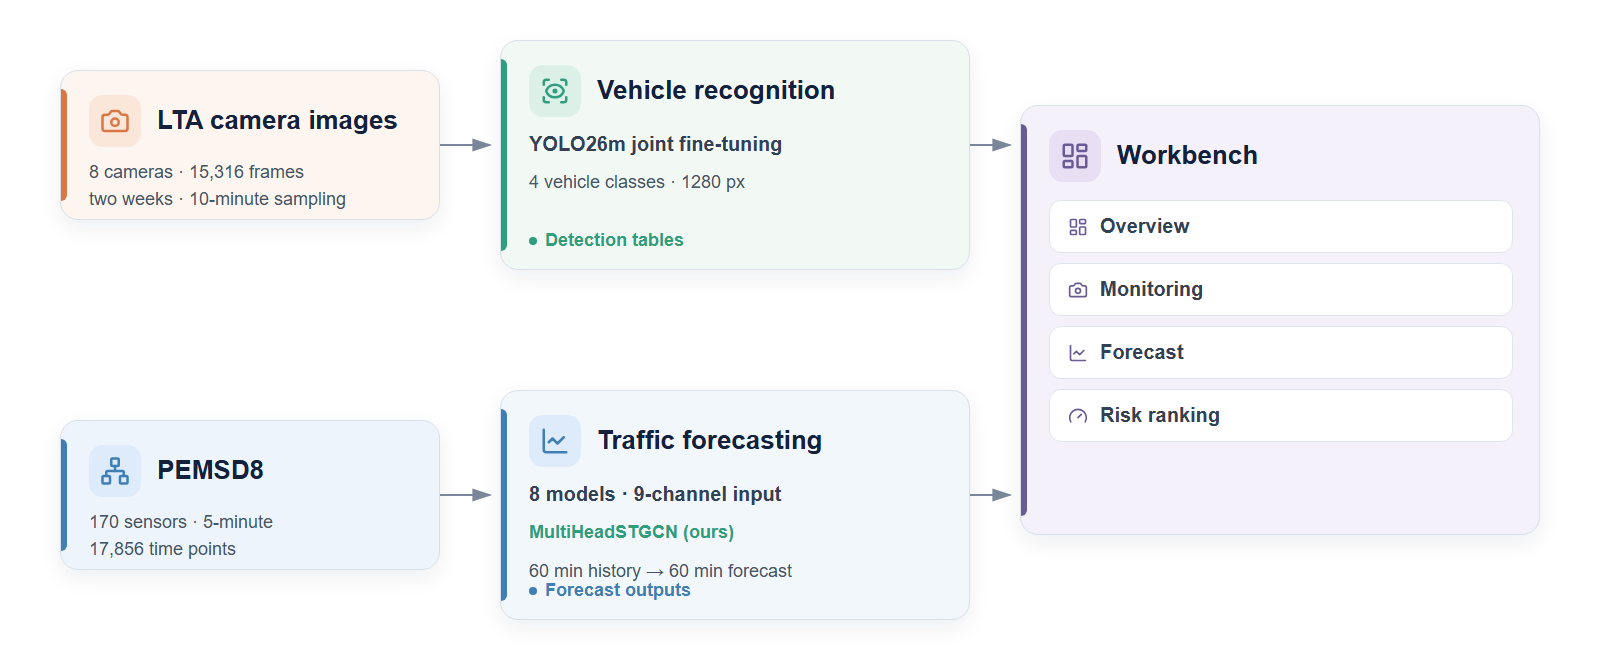
\includegraphics[width=\linewidth]{architecture.png}
  \caption{Prototype architecture. The upper path processes LTA camera images
  for vehicle recognition and its post-processing layers; the lower path
  processes PEMSD8 time series for traffic forecasting. Both outputs feed the
  workbench. The camera-filter and congestion layers are described in
  Section~\ref{sec:method-congestion} and omitted here for clarity.}
  \label{fig:architecture}
\end{figure}

\subsection{Camera Filter and Congestion Estimation}\label{sec:method-congestion}

The joint detector runs on fixed cameras, so many of its false positives recur
at the same image positions: road signs, traffic lights, lane markings and the
central median. A per-camera filter removes them without retraining. Each camera
is calibrated once with three elements in normalized image coordinates: a road
region, an exclusion set and detection zones. A box is kept only if its
bottom-centre point lies inside the road region. It is removed if it matches an
exclusion entry, either when its point lies in the entry (point rule) or only
when the whole box does (box rule), at all times or only by day or night. The
box rule protects vehicles that queue beside a fixed false positive; it is used
for a traffic light at camera 4703, where motorcycles wait next to it.

Calibration uses a browser page that plots the bottom-centre points of two weeks
of detections for each camera and proposes draft polygons from their density. An
annotator adjusts the vertices and accepts or rejects candidate false positives,
which are boxes that recur at the same position. The 80 week-2 validation images
are excluded from calibration, so the human-corrected images in
Section~\ref{sec:results-filter} were held out from calibration. Because the
filter is calibrated per camera, this evaluates image-level correction, not
transfer to new cameras. The filter can wrap the detector as a drop-in
replacement or filter the existing detection table.

The congestion module rates every LTA frame as free-flowing, moderate or
congested, judging only the detection zones: near-field segments that cover the
full width of one direction, drawn in the same calibration step. Three voters
score each frame independently. Voter~A uses the filtered output of the joint
detector: it counts vehicles whose bottom-centre lies in each zone and measures
box occupancy, the share of zone area covered by boxes. Voter~B is classical
image processing: for each camera and hour of day, a per-pixel median over two
weeks gives a background, and Canny edges \parencite{canny1986edge} present in
the frame but not in the background count as foreground, ignoring over-exposed
pixels. The background uses all frames in the collection, including test frames,
but no labels; it is an unsupervised, transductive step. Voter~C applies a
pretrained vision-language model without further
training: OpenCLIP ViT-B/16 trained on a LAION-2B subset of LAION-5B
\parencite{radford2021clip,cherti2023openclip,schuhmann2022laion} compares a
crop around the zones with three groups of text prompts, and its class
probabilities give a congestion score.

When a camera's zones cover two roads, the human label follows the more
congested one, so each voter is computed both over all zones and for the busiest
zone. Five candidate methods are compared: each voter alone with two cut points,
the median of the three voters' levels, and stacking
\parencite{wolpert1992stacking}, a multinomial logistic regression on the log
vehicle count, occupancy and the B and C scores. Features, cut points and the
primary method are chosen on practice labels only
(Section~\ref{sec:setup-metrics}); the frozen primary method then rates all
15,316 frames.

\subsection{Forecasting Module}\label{sec:method-forecasting}

The forecasting module operates on road-network time series. PEMSD8 provides a
calibrated multivariate benchmark with standard evaluation splits: 170 sensors,
five-minute observations, and flow, occupancy and speed measurements. The module
is trained, tested and compared on PEMSD8, which supports multivariate graph
models and comparison with published baselines. The LTA collection provides
per-frame vehicle counts at ten-minute intervals; Section~\ref{sec:method-integration}
defines the calibrated series required to connect these counts to the
forecasting module.

The module compares eight models under a common protocol: FNN, STGCN, MTGNN,
MultiHeadSTGCN, GRU, LSTM, GWNET and AGCRN. The first seven follow their LibCity
implementations; MultiHeadSTGCN is the project's custom model. The set covers
feed-forward, recurrent, fixed-graph, learned-graph and node-embedding designs.
Two input settings are compared: each model's default configuration, and a
unified nine-channel setting (flow plus time-of-day plus day-of-week). The
unified setting controls the information available to each model, but it does
not equalize optimizer, loss function, parameter count or training budget. The
top four models on the unified setting are re-run with seeds 0--4 and compared
with paired differences. Every run records its resolved configuration, data
provenance, training history and checkpoint selection.

MultiHeadSTGCN is based on STGCN and keeps its temporal and spatial blocks. It
changes four aspects. First, it predicts all output steps in one forward pass
instead of the LibCity STGCN implementation's single-step output followed by
autoregressive rolling. Second,
output heads are target-specific: each head produces the complete 12-step
horizon, and a single-target run uses one head. The multi-head capacity is
exercised only when several targets are trained jointly. The benchmark in this
report uses the single-target flow configuration, so its results do not
demonstrate a benefit from multiple heads. Third, it adds time-of-day and
day-of-week inputs. Fourth, it can use either Chebyshev convolution on the
symmetrized PEMSD8 sensor-link adjacency or directed dual-path propagation on
the original directed links. The default configuration uses the symmetric
Chebyshev variant, a collapsed output head that compresses the temporal axis
before the final projection, and the two calendar features.
Section~\ref{sec:results-ablation} quantifies each step.

\subsection{Workbench}\label{sec:method-workbench}

The Traffic Monitoring and Forecasting Workbench is a prototype traffic
monitoring and forecasting system. The product concept is a single operator
workbench that combines camera monitoring, vehicle counts and short-term
congestion forecasts in one interface. The prototype provides three views over
the processed outputs:

\begin{itemize}
  \item \textbf{Overview}: a situation summary, a needs-attention queue, camera
        and forecast health cards, and a camera coverage map.
  \item \textbf{Monitoring}: a camera picker, a time-controlled detection frame,
        camera reliability metrics (frames processed, zero-detection rate, mean
        confidence and completeness), and a per-class count timeline.
  \item \textbf{Forecast}: replay-time and horizon controls, a predicted-severity
        network schematic, an observed and forecast speed curve with an empirical
        residual band, and a threshold-based risk ranking.
\end{itemize}

Figure~\ref{fig:workbench} shows the overview: it combines the source labels for
both data domains, the needs-attention queue, the module health cards and the
camera coverage map. The workbench presents historical replay, and the interface
marks this state. It reads the detection tables and forecast run records, and each view labels
its data source. The Monitoring view shows
processed frames from the LTA collection; the Forecast view uses PEMSD8 and
identifies its sensors as belonging to a public California road network,
separate from the LTA cameras. The workbench is implemented as a lightweight web
application with static HTML, CSS and JavaScript for the interface and a Python
service for data access and consistency checks.

\paragraph{Congestion risk estimation.}
The Forecast view uses the speed-target run rather than the flow benchmark,
because the risk indicator is defined on speed. Detectors are classified as
watch below 55 mph, congested below 45 mph and severe below 35 mph. These
thresholds are operational choices anchored to a test-period free-flow median of
about 65 mph; they are not a traffic-engineering standard. For each detector, the
interface takes the worst predicted speed over the selected horizon, including
the current observation, and ranks detectors by severity, status and onset. The
result is a threshold-based risk indicator intended for comparative
visualization, not a validated congestion estimate. The shaded band is the
10th--90th percentile of per-detector residuals on the test period, an empirical
error range rather than a calibrated prediction interval.

\paragraph{Camera filter and congestion layers.}
The Monitoring view also shows two layers that read the outputs of
Section~\ref{sec:method-congestion}. A camera-filter switch dims the area outside
the road region, outlines the detection zones and draws the removed boxes with
their reason, and the reliability panel reports the share of boxes removed for
the camera. Each frame shows its congestion level, and a weekday-by-hour heatmap
gives the share of congested frames for the selected camera together with its
test-set accuracy. Without these outputs the view is unchanged. This congestion
level describes the LTA camera view; it is separate from the speed-based risk
indicator above, which is defined on PEMSD8.

\begin{figure}[t]
  \centering
  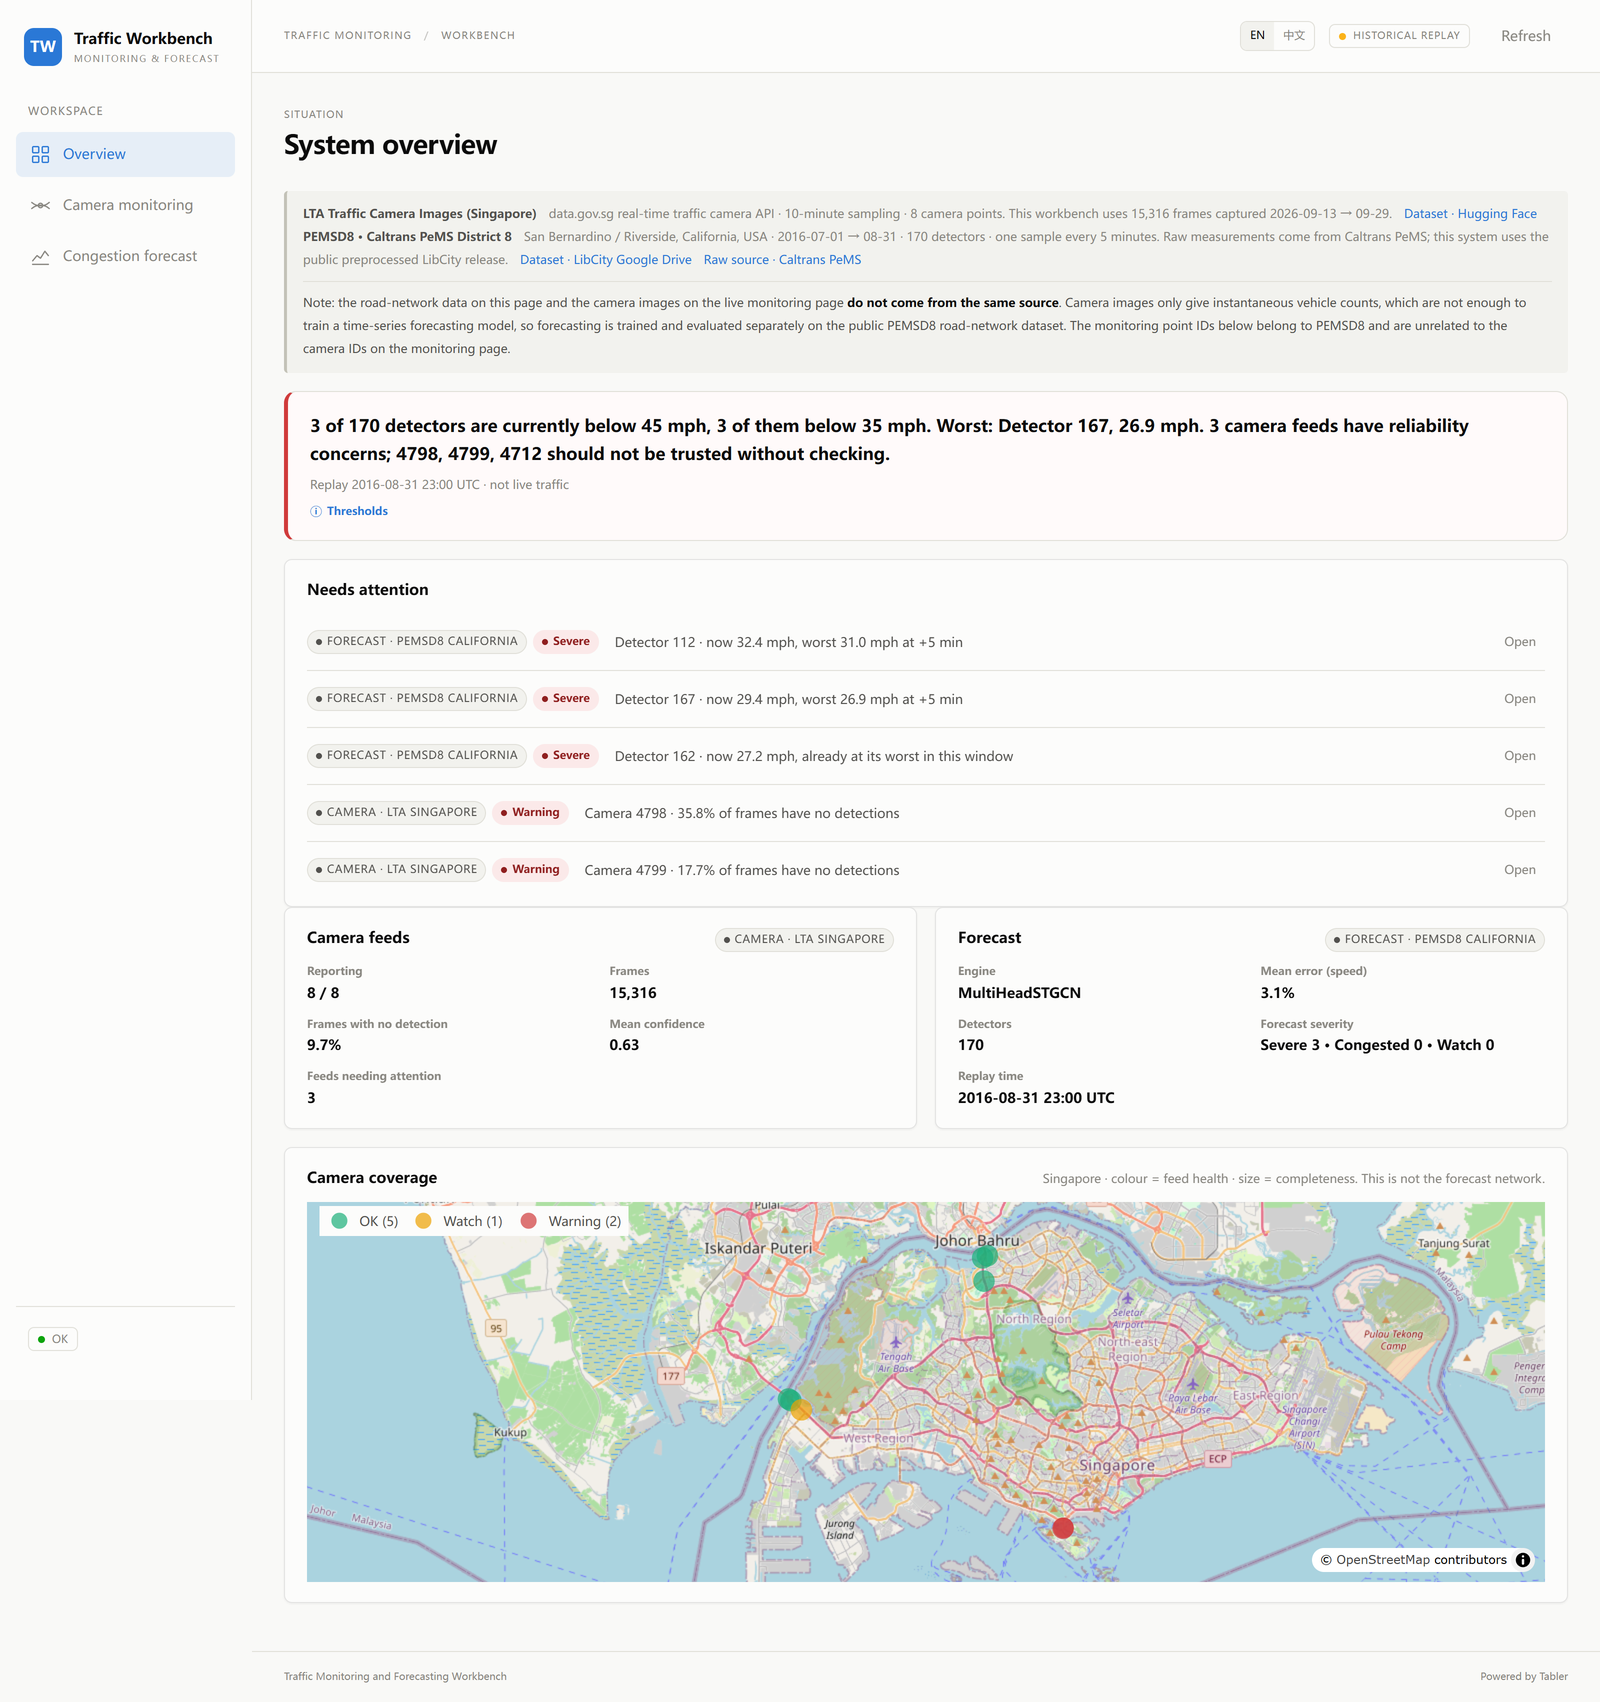
\includegraphics[width=0.92\linewidth]{workbench_overview.png}
  \caption{Workbench overview. Each view labels its data source. The page lists
  forecast and camera items that need attention, summarizes module health, and
  maps the eight LTA camera feeds.}
  \label{fig:workbench}
\end{figure}

\subsection{Implementation and Evaluation Tools}\label{sec:method-tools}

The detection module uses Ultralytics YOLO26 \parencite{ultralytics2026yolo} on
PyTorch \parencite{paszke2019pytorch}, with OpenCV and Pillow for image handling.
Fine-tuning and evaluation follow the MIO-TCD protocol
\parencite{luo2018miotcd}. The project code, workbench, experiment scripts and
run records are available in the repository.\footnote{The code revision used for
the reported runs is the \texttt{develop} branch:
\url{https://github.com/LOVEIII486/ISY5002-TrafficPrediction/tree/develop}}
The forecasting module uses LibCity \parencite{wang2021libcity,jiang2023libcity},
PyTorch, NumPy, pandas and SciPy.\footnote{LibCity code:
\url{https://github.com/LibCity/Bigscity-LibCity}} The workbench uses Python with
static HTML, CSS and JavaScript (Tabler components).\footnote{\url{https://tabler.io/}}
The camera filter and the congestion module use OpenCV, scikit-learn and
OpenCLIP \parencite{cherti2023openclip}.
Large prediction arrays and trained weights are not stored in version control;
the benchmark commands regenerate the arrays consumed by the workbench. The
human-corrected LTA annotations, manifests and COCO/YOLO exports are released in
\texttt{datasets/lta\_human\_v1}; images are referenced by filename and SHA-256
rather than redistributed. Detection accuracy is measured with COCO-style mAP
\parencite{lin2014coco}, and uncertainty is estimated with bootstrap resampling
\parencite{efron1993bootstrap}.

\subsection{Integration Design}\label{sec:method-integration}

The prototype is organized as three top-level modules with a shared workbench;
the camera filter and congestion estimate are recognition post-processing layers,
not additional data domains. A fully
integrated deployment requires a calibrated, time-aligned traffic series at the
camera locations. LTA images provide instantaneous vehicle counts; a forecasting
model additionally needs a consistent series of flow, and ideally occupancy and
speed, over weeks or months. The integration design has three steps. First,
calibrate camera counts against a trusted volume source and aggregate them to
fixed intervals. Second, obtain flow, occupancy and speed series for the same
locations and align their timestamps with the image feed. Where the existing
camera view is too distant or poorly lit, close-range cameras or dedicated
traffic sensors can provide clearer measurements. Third, train the forecasting
module on the local series and connect both modules to one data domain in the
workbench. This design defines the interface between the two modules
and the measurements required to complete it.
